%==========================================================================
\chapter{Documentation Standards}
\label{Documentation Standards}

All documentation is available on the Scalable Linear Solvers Members Only
webpage in HTML format.  You can also get postscript version from the
repository (in the docs directory).  Both of these are updated daily since
autotest builds the docs directory every night. 
\newline
To add/update documentation do the following:
\newline
To add to the Users Manual or Developers Manual create a Latex file and
prepend 
\begin{verbatim} usr_ \end{verbatim}
to the 
filename.  In the file use the chapter and label conventions following in
other 
\begin{verbatim} usr_*.tex \end{verbatim} 
files.  Then add this file to 
\begin{verbatim} usr_manual.tex \end{verbatim} 
in the 
``Include Chapters'' section.  Both this change and the new latex
file must be committed.  
\newline\newline
To add to the Code Reference Manual DOC++ must be used.  The first step is
to add DOC++ style comments to your source code in source.c.  The CASC software development web page has information on how to do this.  When the docs 
directory is built, these comments will be put into a file called
source.dxx.  Next, add a file to the docs
directory (or use an existing one if applicable-- currently the sections
are divided into ``Interface Reference'' and ``Implementation Reference'') 
called 
\begin{verbatim} filename_ref.dxx. \end{verbatim} 
Examine additional targets in the Makefile if you want to build only
certain parts of the documentation.  If creating a new one, follow the 
conventions used in \begin{verbatim} interface_ref.dxx \end{verbatim} and be sure to include it in 
\begin{verbatim} code_ref.dxx. \end{verbatim}  
In the new (or existing) .dxx file include 
source.c for all newly documented source files, including full path name. 
\newline\newline
To build documentation go into the docs directory and type ``make''.  
Examine additional targets in the Makefile if you want to build only
certain parts of the documentation.   If you are adding or changing any
documentation please check to make sure it builds correctly prior to 
committing it to the repository-- if the build breaks then the online 
documentation will not be available to anyone on the following day. You will
find the html files in automatically created directories called 
\begin{verbatim} docs/HYPRE_dev_manual and docs/HYPRE_usr_manual and docs/HYPRE_code_ref.\end{verbatim}

Example documentation for C routines can be found in the directory
\file{struct_matrix_vector} in the files:
\begin{verbatim}
   communication.c
   communication_info.c
   computation.c
\end{verbatim}

%==========================================================================
\section{Example of Figure Use}
\label{Example of Figure Use}

Here is an example of how figures might be used.  Here we want to
illustrate how a figure is included in both the printed manual and the
online manual.  So, see Figure \ref{fig-conceptual-interface}.  The
\code{figure} environment is automatically converted to a GIF image by
LaTeX2HTML, so graphics included this way need only exist in
postscript format.
\begin{figure}
\centering
\includegraphics[width=5in]{concep_iface.eps}
\caption{%
Graphic illustrating the notion of conceptual interfaces.}
\label{fig-conceptual-interface}
\end{figure}

To insert graphics that are not figures (i.e., not in a figure
environment), where both a \code{.eps} and a \code{.gif} file have
already been created, use the macro \code{InsertGraphics}.  This
produces the following:

\begin{center}
\InsertGraphics{hypre_wiw}{width=5in}
\end{center}
